\documentclass[10pt]{article}
\usepackage[utf8]{inputenc}
\usepackage{tikz}
\usepackage{pgfplots}
\usepackage{pdflscape}
\usepackage{geometry}
\pgfplotsset{compat=1.18}

\pagestyle{empty}

\geometry{
    top=25pt,
    bottom=1pt,
    left=1pt,
    right=1pt
}

\begin{document}

\begin{landscape}
    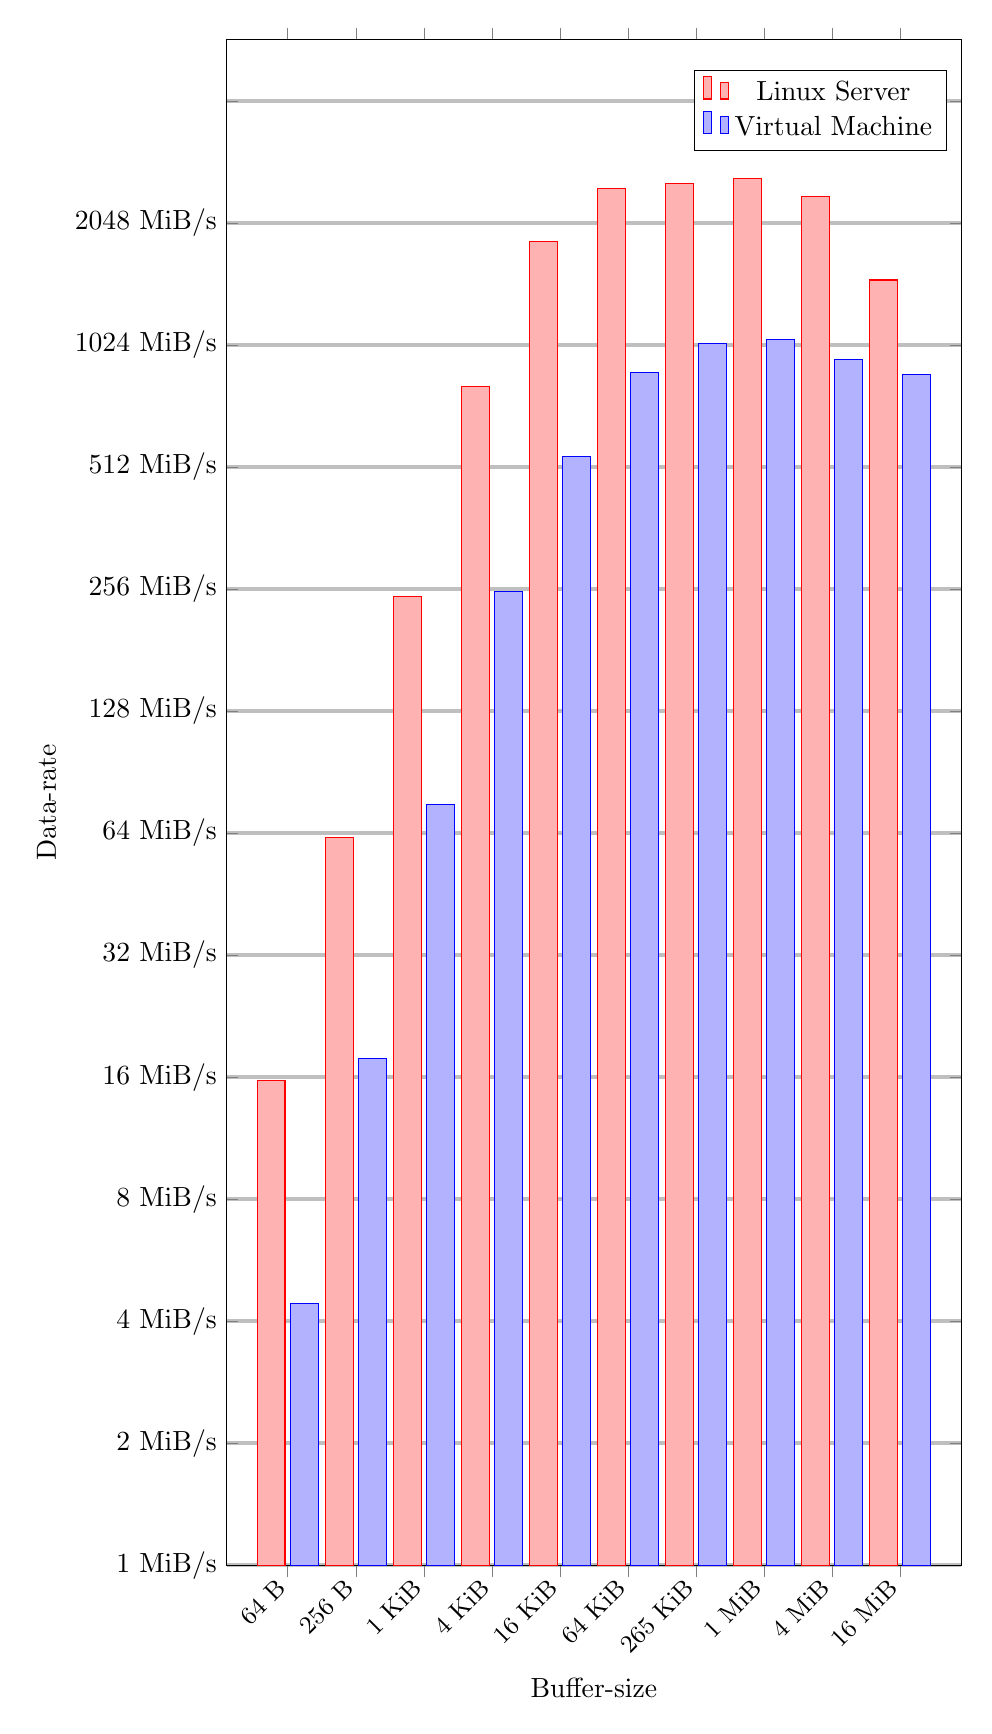
\begin{tikzpicture}
        \begin{axis}[
                ybar,
                xmode=log,
                ymode=log,
                log basis x={4},
                log basis y={2},
                width=0.9\linewidth,
                height=0.75\pdfpageheight,
                xlabel=Buffer-size,
                ylabel=Data-rate,
                xticklabels={0, 64 B, 256 B, 1 KiB, 4 KiB, 16 KiB, 64 KiB, 265 KiB, 1 MiB, 4 MiB, 16 MiB},
                yticklabels={1 MiB/s, 2 MiB/s, 4 MiB/s, 8 MiB/s, 16 MiB/s, 32 MiB/s, 64 MiB/s, 128 MiB/s, 256 MiB/s, 512 MiB/s, 1024 MiB/s, 2048 MiB/s},
                x tick label style={rotate=45, anchor=east, font=\small},
                ymin=1,
                ymajorgrids=true,
                major grid style={line width=1.5pt}
            ]

            \addplot[red, fill=red!30] coordinates {
                    (64, 15.68) (256, 62.47) (1024, 244.91) (4096, 809.71) (16384, 1843.20) (65536, 2490.99)
                    (262144, 2558.85) (1048576, 2634.28) (4194304, 2378.18) (16777216, 1479.20)
                };
            \addplot[blue, fill=blue!30] coordinates {
                    (64, 4.42) (256, 17.74) (1024, 75.31) (4096, 251.60) (16384, 542.94) (65536, 873.51)
                    (262144, 1030.14) (1048576, 1056.04) (4194304, 940.53) (16777216, 866.51)
                };
            \legend{Linux Server, Virtual Machine}
        \end{axis}
    \end{tikzpicture}
\end{landscape}
\end{document}